%\chapter{Introduction}
%already present in the main file

\graphicspath{{../img/ch10/}}


Four separate topics are presented in the present thesis and the discipline of Information Extraction is the central point of them. Each topic represents one particular aspect of the Information Extraction discipline.

The first two topics are focused on our information extraction methods based on deep language parsing. The first topic relates to how deep language parsing was used in our first method in combination with manually designed extraction rules.

The second topic deals with an alternative extraction method based on machine learning. An inductive procedure was developed based on Inductive Logic Programming, which allows automated learning of extraction rules from a learning collection.

The idea of the Semantic Web was the strongest motivation of our research from the very beginning. We wanted to exploit information extraction techniques to speed up the semantic web evolution. The third topic of the thesis presents even more than that. The core of the extraction method was experimentally reimplemented using semantic web technologies. Therefore not only the result of information extraction but also the extraction procedure itself is realized using semantic web technologies. The main advantage of this approach is the possibility to save the extraction rules in so called shareable extraction ontologies.

The last topic of this thesis is the most distant from the original information extraction topic. We have included it because it represents an important part of our research and considerable effort was spent on it. The topic deals with document classification and fuzzy logic. We are investigating the possibility of using information obtained by information extraction techniques to document classification. Our implementation of so called Fuzzy ILP Classifier was experimentally used for the purpose of document classification.

\section{Motivation}
The basic motivation of our research can be illustrated with three images or schemas that are presented in Figures~\ref{fig:acquisitions_annotated}, \ref{fig:fireman_annotated} and \ref{fig:intro_damage_tree}. The first two figures show some texts with several pieces of information decorated in it. If you show such images to a human, he or she will be shortly able to find such pieces of information in any other text of the same kind. But can this relatively simple task do a computer as well? Figure~\ref{fig:intro_damage_tree} represents our first ideas when we started to look for the answer. The figure shows a linguistic tree obtained by automated linguistic analysis of the last sentence of the second figure (Figure~\ref{fig:fireman_annotated}). It already contain lots of indications (decorated with orange tags) of where to look for the wanted piece of information, in this case, the amount of 8,000 Czech Crowns representing the total damage sought by the accident reported in the text.


\begin{figure}
\centering
\framebox{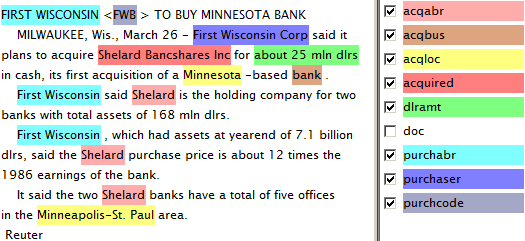
\includegraphics[width=0.75\hsize]{acquisitions_annotated}}
\caption{Corporate Acquisition Events annotations}
\label{fig:acquisitions_annotated}
\end{figure}


\begin{figure}
\centering
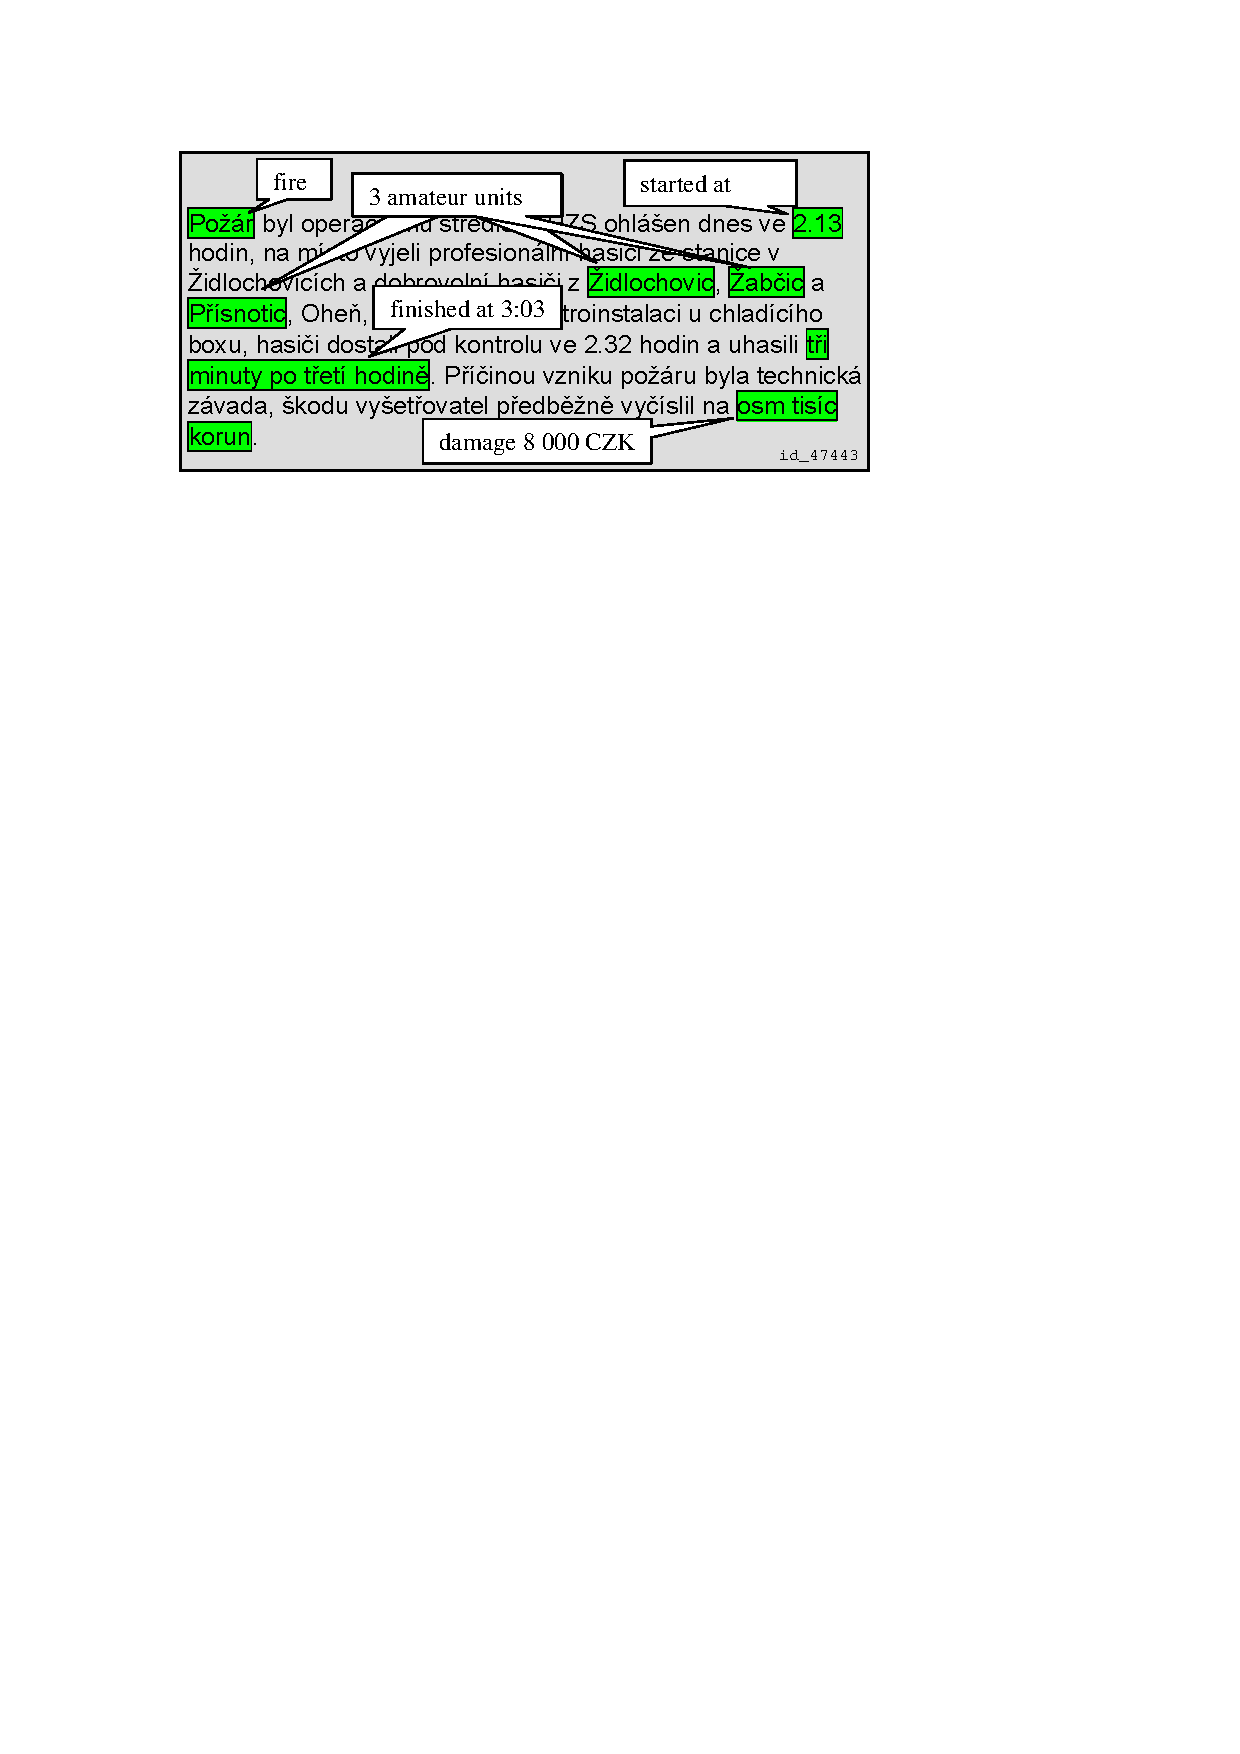
\includegraphics[width=0.65\hsize]{fireman_annotated}
\caption{Fireman Events annotations}
\label{fig:fireman_annotated}
\end{figure}


\begin{figure}
\centerline{\framebox{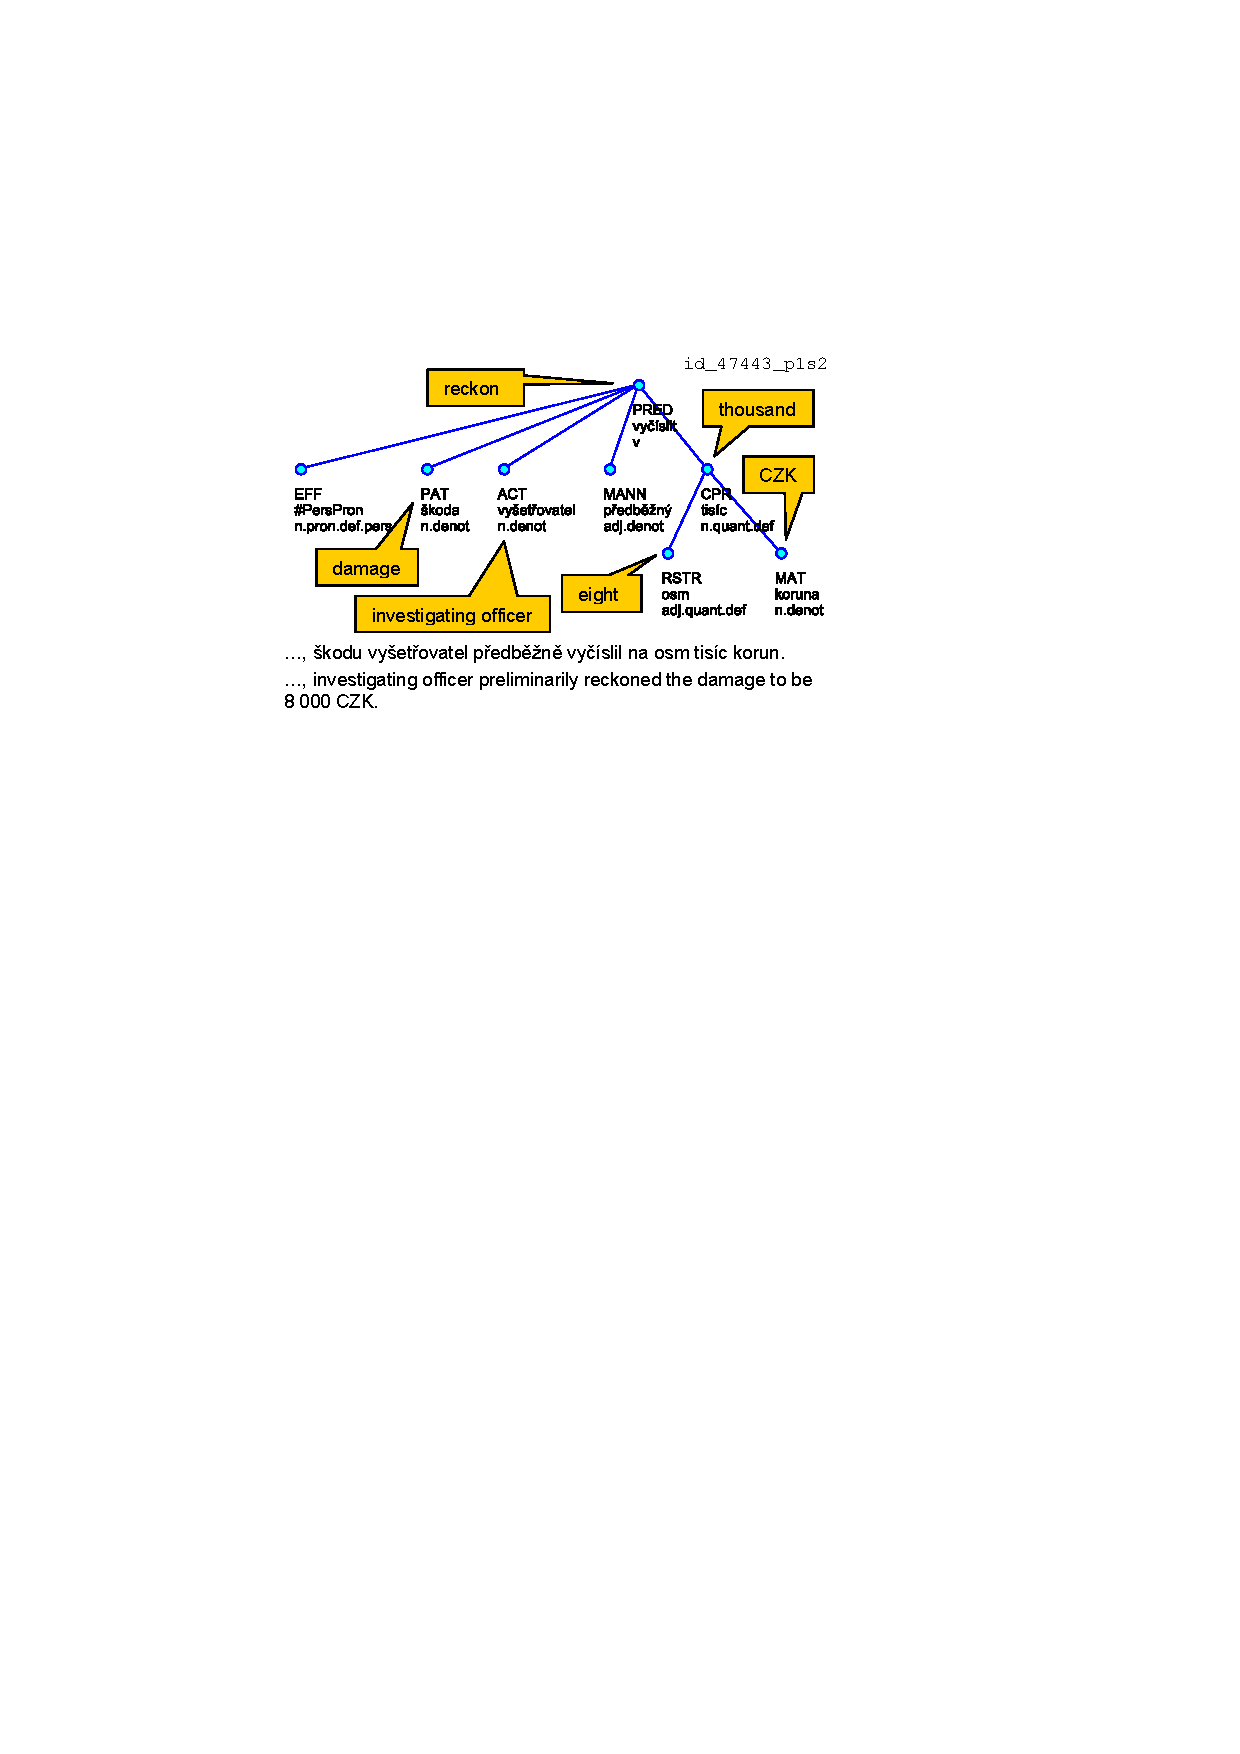
\includegraphics[width=0.7\hsize]{damage_tree}}}
\caption{Example of a linguistic tree of one analyzed sentence.}
\label{fig:intro_damage_tree} 
\end{figure}


%\subsection{Motivation of Our Approaches}

The main motivation for creating our extraction methods was an attempt to use deep linguistic analysis for this task. Especially for the Czech language with free word order this seemed reasonable. It is much more straightforward to design extraction rules on the basis of linguistic dependency trees than to struggle with the surface structure of text. In a dependency tree, the position of a word is determined by its syntactic (analytical trees) or even semantic role (tectogrammatical trees). So the extraction rules might not be dramatically affected by minor variations of the word order.

%\subsection{Usage}
Besides that information extraction and annotation is very interesting and challenging problem, it is also particularly useful. This period can be characterized by information overload and information extraction can provide partial answer to that. It provides fine grained indexing of documents, which supports precise search and document filtering. Navigation within individual documents can be faster and reading can be more effective. Other software programs can use the extracted information and perform additional computations resulting in summaries and answers integrated from different sources.  The effort in this direction will hopefully culminate in the realization of the idea of the Semantic Web, when all the information will be available in a machine workable form and the whole (semantic) web could be used as a huge knowledge base.



\section{Main Goals and Contributions}

To be written!!!

----

The main \emph{contributions} presented in this chapter are \emph{formal models}, prototype \emph{implementation} and experimental \emph{evaluation} of the Fuzzy ILP Classifier.



\section{Organization}

Rather than presenting individual topics or approaches of this thesis separately in distinct chapters, we decided to organize this document according to common aspects of these approaches and to dedicate individual chapters to these aspects instead of individual approaches. This way, all the (four) approaches are described in parallel in each chapter. 

Chapter~\ref{sec:ch_problems} provides definitions of the individual problems and consequent tasks solved in this thesis.
Chapter~\ref{sec:ch_related} contains description of the most related work of other scientists.
Chapter~\ref{sec:ch_third_party} introduces the most important third party tools and resources that were used in our research.
Chapter~\ref{sec:ch_methods} describes solutions, used models and methods of the individual approaches presented in this thesis.
Chapter~\ref{sec:ch_implementation} provides details about implementation of all the approaches.
Chapter~\ref{sec:ch_data} describes all datasets that were used in our experiments.
Chapter~\ref{sec:ch_eval} describes all experiments that we performed mostly for evaluation of the approaches.
Finally, Chapter~\ref{sec:ch_conclusion} concludes the thesis.

